\documentclass[10pt, a4paper]{article}
\usepackage[slovene]{babel}
\usepackage[utf8]{inputenc}
\usepackage{lmodern}
\usepackage[T1]{fontenc}
\usepackage{eurosym}
\usepackage{amssymb}
\usepackage{amsfonts}
\usepackage{amsmath}
\usepackage{graphicx}
\usepackage{amsthm}

\begin{document}


\begin{titlepage}
\begin{center}
\vspace*{1cm}

\Large
Finančni praktikum - kratka predstavitev

\vspace{0.5cm}
\LARGE
\textbf{Tabu search on TSP}

\vspace{1.5cm}
\Large
Andraž Mur \\
Max Filip Uršič

\vspace{3cm}

\includegraphics[scale=1]{logo}


\vfill

\large Ljubljana, december 2018

\end{center}
\end{titlepage}


\section{Uvod}

Metodo Tabu search je ustvaril Fred W. Glover leta 1986, natančneje pa jo je formaliziral leta 1989. Gre za metaheoristično iskalno metodo, ki se uporablja v matematični optimizaciji.

Kot najbrž vsi vemo, lokalne optimizacijske metode delujejo na način, da za začetni problem poiščejo neko rešitev in nato v okolici te rešitve iščejo izboljšano rešitev in se v primeru, ko boljše rešitve v tej okolici ni, zaključijo. Zaradi tega se pogosto zgodi, da se te metode zaključijo v neki rešitvi, ki ni optimalna, npr. v lokalnem ekstremu.

Tabu search izboljša delovanje takšnih metod tako, da sprosti njihovo osnovno načelo delovanja. Na vsakem koraku namreč dovoljuje slabše korake, torej iskanje rešitev, ki so slabše od trenutno optimalne, če boljših rešitev v okolici ni mogoče najti. Poleg tega upošteva tudi prepovedi v iskanju, kar preprečuje vračanje v že prej obiskane rešitve.

Implementacija tabu search-a uporablja spominske strukture, ki opisujejo že obiskane rešitve ter neka začetna pravila. Potencialna rešitev, ki je bila v bližnji preteklosti že obiskana ali krši kakšno od začetnih pravil, je označena kot ''tabu rešitev'', zato je algoritem v prihodnosti ne upošteva več.




\section{Tabu search in problem potujočega trgovca}

Pri problemu potujočega trgovca se nam porodi naslednje vprašanje: Katera je najkrajša pot, ki obišče vsako mesto in se na koncu vrne v začetno mesto, če imamo podan seznam mest ter razdalje med njimi? To je NP težak problem, katerega število korakov v najslabšem primeru narašča tako hitro z naraščanjem števila mest, da se ga ne da omejiti z nobenim polinomom (a ne eksponentno hitro). Problem je v praksi uporaben na več področjih, med katerimi so najbolj znana logistika, planiranje ter proizvodnja mikročipov. Malo modificiran problem pa se uporablja tudi v sekvencioniranju DNA, kjer »mesto« predstavlja različne dele DNA-ja in »razdalja« predstavlja podobnost med le-temi. Problem potujočega trgovca se uporablja tudi v astronomiji, kjer astronomi poizkušajo minimizirati čas, porabljen za premikanje teleskopov med mesti, iz katerih želijo opazovati vesolje.

\begin{center}
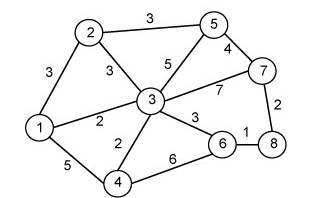
\includegraphics[scale=0.5]{slika1}
\end{center}

Uporaba metode tabu search na opisanem problemu deluje na način, ki sva ga opisala v uvodu. Na začetku moramo poiskati neko rešitev danega problema, kar je v praksi precej enostavno. Poiščemo jo lahko na način, da se iz vsakega vozlišča pomaknemo v eno od sosednjih vozlišč, ki še ni bilo obiskano. Za tem v okolici te rešitve iščemo njeno izboljšavo, torej moramo najprej sploh definirati okolico rešitve.

Okolica neke rešitve problema je definirana kot katerakoli druga rešitev problema, ki jo dobimo z zamenjavo dveh vozlišč v trenutni rešitvi. To nam zagotavlja, da so vsi elementi okolice res rešitve našega problema. Ker želimo preprečiti, da bi se metoda vračala v že prej obiskane rešitve, moramo seveda definirati tudi tabu seznam za rešitev. Na ta seznam bomo zato uvrstili vsako rešitev, ki je bila prepoznana kot element neke okolice prejšnjih rešitev. Upoštevati moramo tudi dejstvo, da je včasih tabu kriterij premočan, zato na vsakem koraku dovoljujemo uporabo neke rešitve z boljšo vrednostjo od trenutno optimalne, tudi če leži v tabu seznamu.

Včasih se proces ustavi v lokalnem optimumu, kar pa za nas ni vedno optimalno, saj ne velja nujno, da je lokalni optimum tudi globalni. Zato je potrebno procesu dovoliti, da razveja svoje iskanje tudi drugam, kar se da narediti s pomočjo frekvenčnega spomina. Ta tistim premikom, pri katerih se rešitev ne izboljša, pripiše neko "kazen" (števec pogostosti, ki je prilagojen za določen faktor). Opisan proces, imenovan diverzifikacija, se uporablja samo, kadar ne obstaja noben premik, ki bi rezultat izboljšal (t.j. ko smo v lokalnem ekstremu). Posledično se informacija o pogostosti uporabi, da proces začne raziskovati prej najmanjkrat obiskane poti in na ta način razširi proces v neraziskane dele.

Algoritem se zaključi, ko je doseženo na začetku določeno maksimalno število korakov iteracije.




\section{Načrt nadaljnjega dela}

Do sedaj sva si torej podrobno ogledala obravnavan problem ter ga poskušala čim bolje razumeti, v prihodnje pa se bova osredotočila na zapis programa, ki bo reševal ta problem. Namen imava napisati program, ki bo s pomočjo tabu search metode za katerikoli problem potujočega trgovca poiskal čim bolj optimalno rešitev. Za programiranje takšnega programa bova najverjetneje uporabljala programski jezik python, vendar dopuščava možnost, da se izbira jezika iz praktičnih razlogov spremeni.

Na koncu naloge pa bova na spletu poizkusila poiskati nekaj uporabnih primerov problema potujočega trgovca in jih rešila s pomočjo najinega programa. V kolikor nama ne bo uspelo najti dovolj primerov ali pa se nama bodo najdeni primeri zdeli neprimerni, si jih bova izmislila sama ali pa bova uporabila kakšnega od primerov, ki smo jih lansko leto rešili pri predmetu Operacijske raziskave. Dobljene rešitve bova nato seveda tudi primerjala z dejanskimi optimalnimi rešitvami primerov.






\end{document}